\section{Umsetzung}

\begin{itemize}
	\item Ausgewählte Implementierungsdetails (Bsp. Algorithmen, Datenstrukturen, Libraries, Architectural Hot Spots)Dokumentation Architektur und Design (i.d.R. plattformneutral bzw. technologieübergreifend, z.B. in Form von UML-Diagrammen und Erläuterungen dazu)
	\item Dokumentation, welche Experimente/Tests durchgeführt wurden und welche Lösungsoptionen aufgrund der Ergebnisse dieser Experimente/Tests verworfen wurden.
\end{itemize}

\subsection{Labor Netzwerk Architektur} \label{subsec:Labor-Netzwerk-Architektur}
Mit der zur Verfügung gestellten Hardware ist die folgende Netzwerk Architektur entstanden.

Folgende zentrale Überlegungen sind eingeflossen:

\begin{itemize}
	\item Campus Netzwerk mit mehreren Gebäuden, um das Wandern von Geräten zu simulieren.
	\item Mischung der zur Verfügung stehenden Switches (Catalyst 9300 \& 3850) in der Fabric Edge Nodes, um Verhalten zu vergleichen.
	\item Management Netzwerk ist inbound. Kabelführung zu jedem Switch ist meistens von den Gegebenheiten in typsichen Gebäuden nicht möglich.
\end{itemize}


\begin{figure}[H]
	\centering
	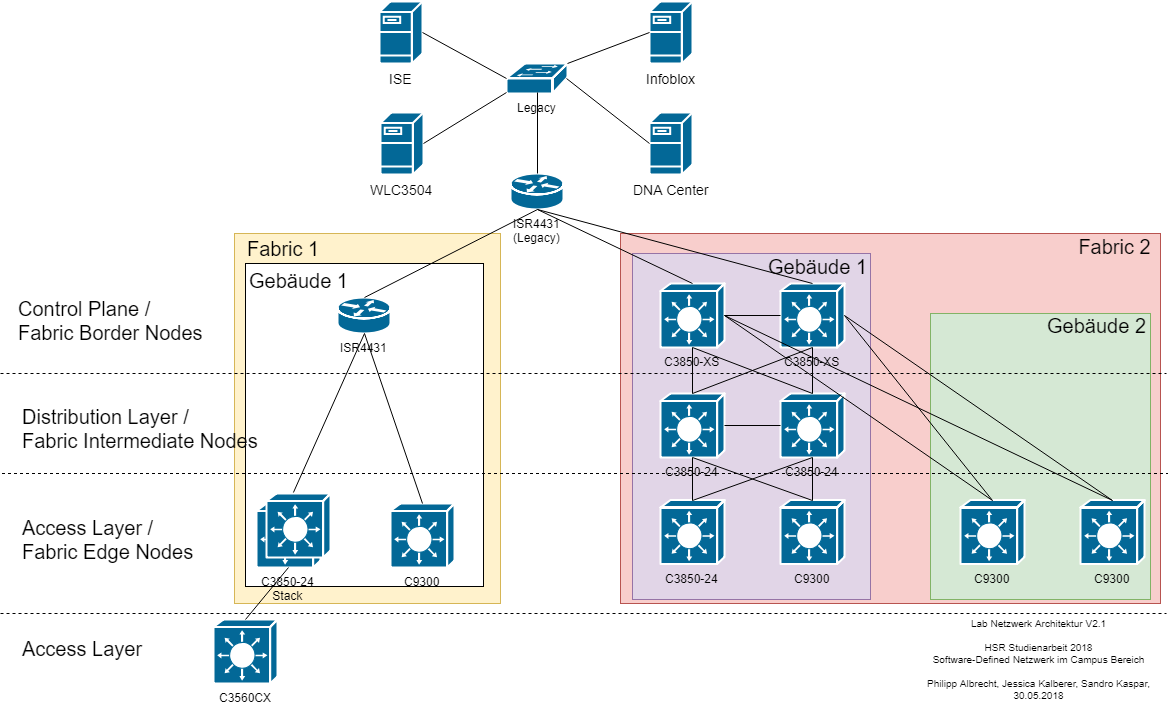
\includegraphics[width=1\linewidth]{img/LabNetworkArchitecture.png}\\[1px]
	\caption{SDN Netzwerk Architektur}
	\label{fig:LabNetworkArchitecture}
\end{figure}

\subsection{Netzwerkarchitekturen Vergleich}
Hauptunterschiede zwischen der klassischen Netzwerkarchitektur und der "Modernen" Software-Defined Access Architektur. 

\begin{itemize}
	\item Bis zur Fabric Edge Nodes (Vergleichbar mit dem Access Layer) unterliegt ein Layer 3 Netzwerk. 
	\item Kein Einsatz von STP oder VSS auf Distribution Layer notwendig, da das Underlay Netzwerk rein Layer 3 ist und Routing Protokolle (OSPF) zum Einsatz kommen.
	\item Der Distribution Layer nimmt neu als Fabric Intermediate Nodes nur noch die Funktion als Layer 3 Brücke bzw. VXLAN transporteuer ein, anstatt die Grenze zwischen Layer 3 und Layer 2 zu sein. Die Fabric Intermediate Nodes sind optional. 
	\item Während beim klassischen Design die logische Netzwerkarchitektur direkt Abhängig ist von der physikalischen Architektur, wird bei SDN die phykalische Netzwerkarchitektur von der logischen Architektur getrennt. Man spricht dann von der Physical Fabric Topology bzw. Underlay und den entsprechenden Layer 2 bzw. Layer 3 Overlay Network. 
\end{itemize}

\begin{figure}[H]
	\centering
	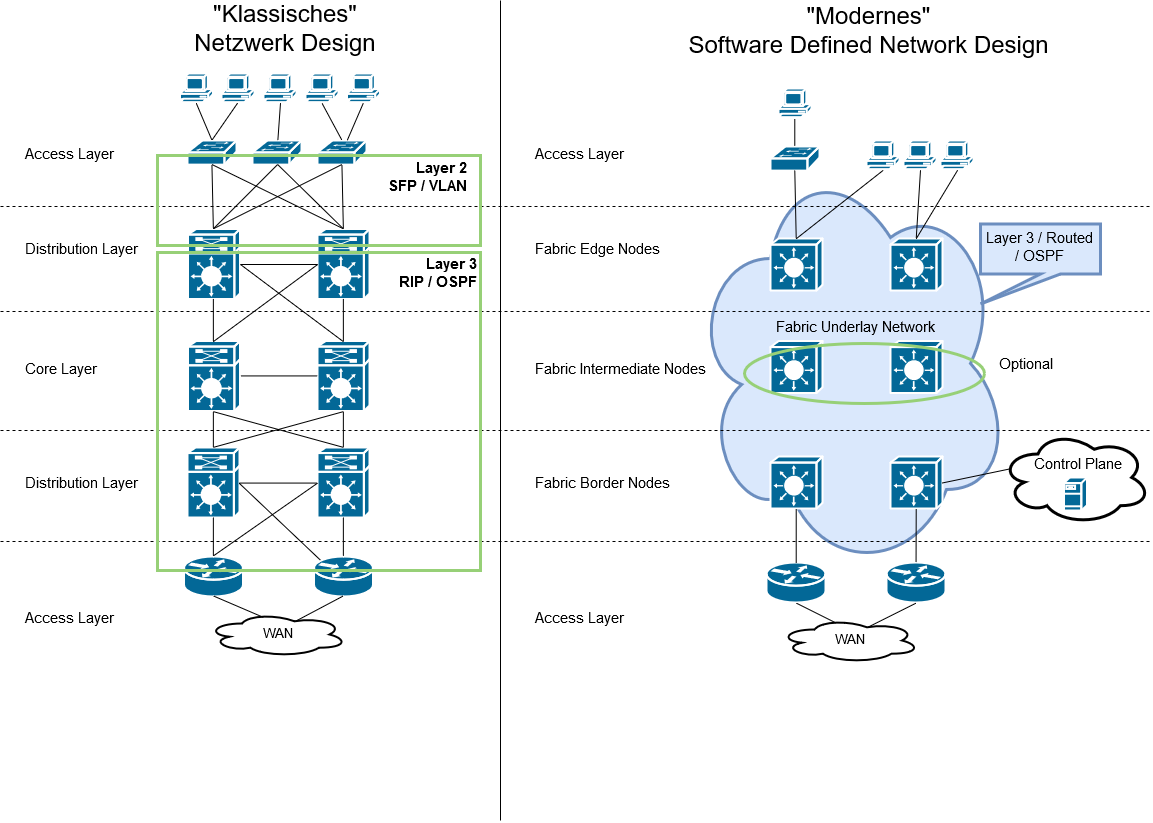
\includegraphics[width=1\linewidth]{img/LabNetworkArchitecture_Vergleich.png}\\[1px]
	\caption{Netzwerk Architektur Vergleich}
	\label{fig:LabNetworkArchitectureVergleich}
\end{figure}

\subsection{Maximale Skalierungen}
Nachfolgend werden die aktuell maximalen Skalierungen des DNA Centers, sowie der Border und Edge Nodes aufgelistet.
\begin{figure}[H]
	\centering
	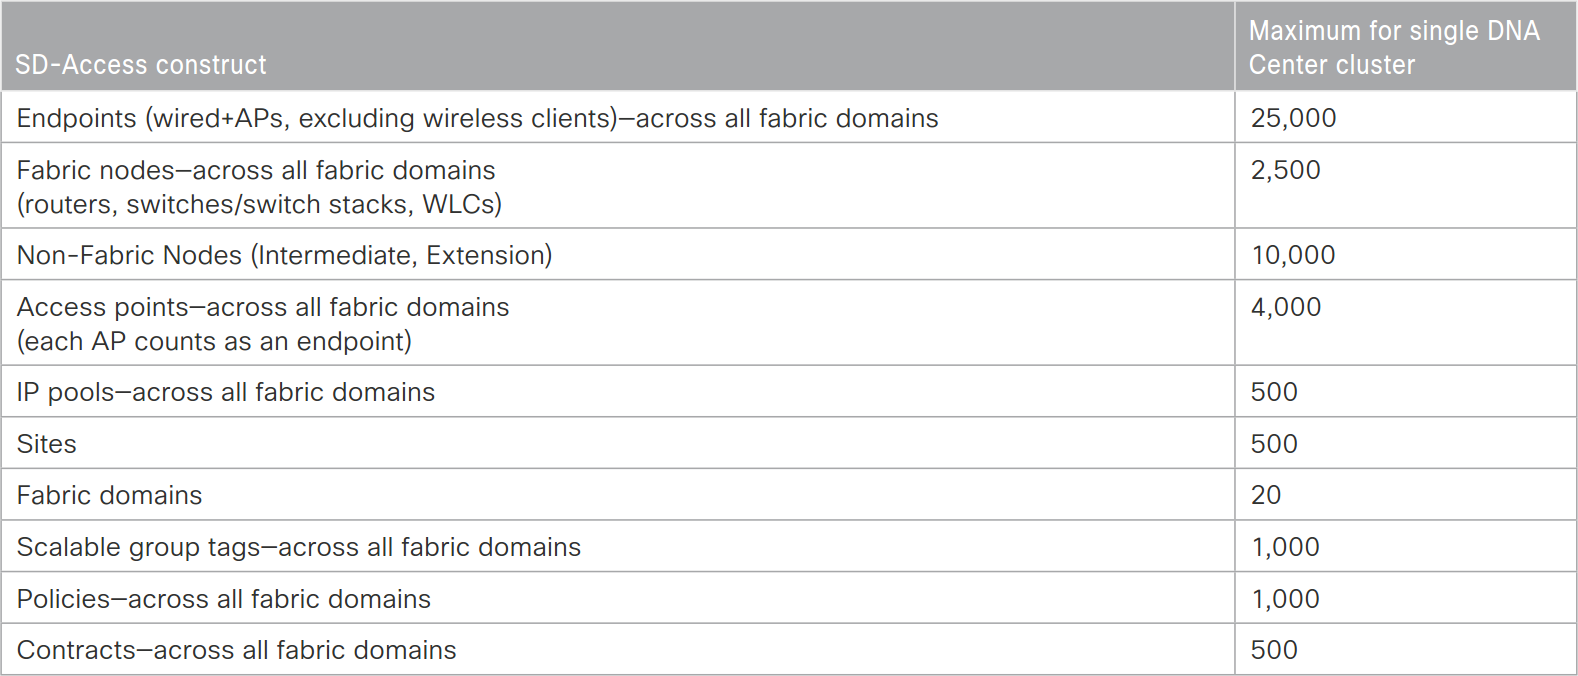
\includegraphics[width=1\linewidth]{img/MaximumScale-HACluster.png}\\[1px]
	\caption{DNA Center Maximum Scale Constraints HA Cluster}
	\label{fig:Maximum Scale HACluster}
\end{figure}

\begin{figure}[H]
	\centering
	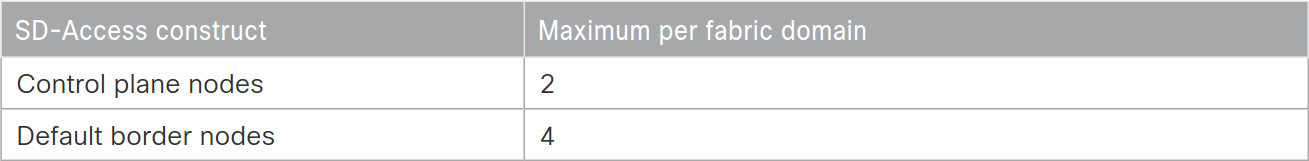
\includegraphics[width=1\linewidth]{img/MaximumScale-Fabric.png}\\[1px]
	\caption{DNA Center Maximum Scale Constraints Fabric}
	\label{fig:Maximum Scale Fabric}
\end{figure}

\begin{figure}[H]
	\centering
	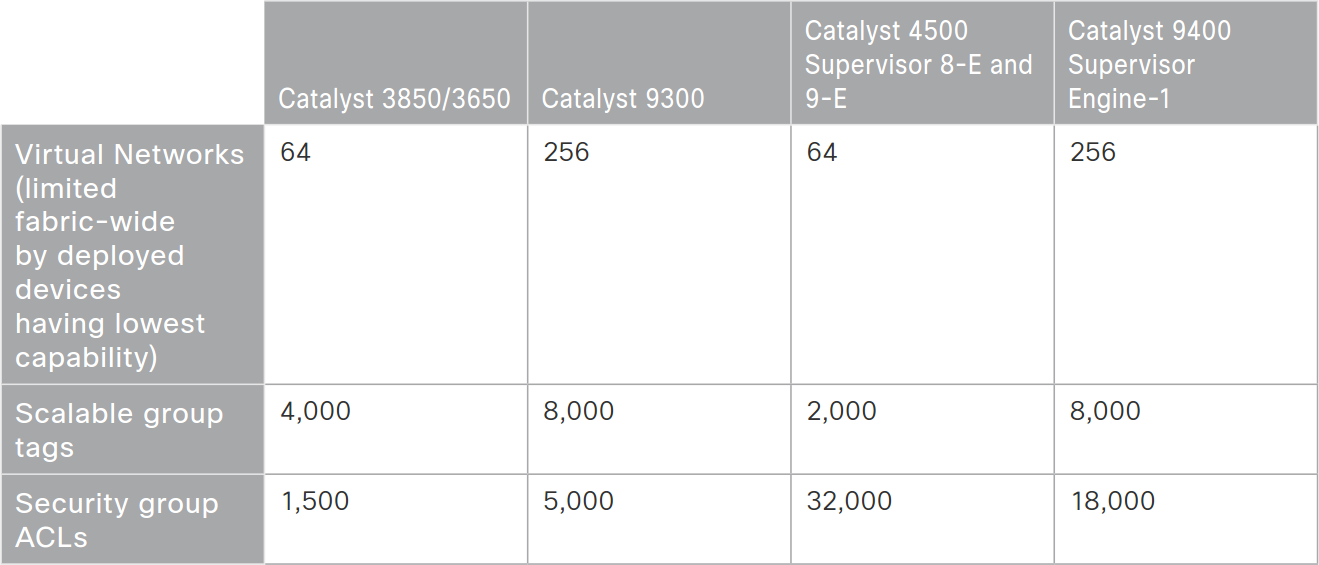
\includegraphics[width=1\linewidth]{img/MaximumScale-EdgeNode.png}\\[1px]
	\caption{SDA Edge Node Scale Constraints}
	\label{fig:SDA Edge Node Scale Constraints}
\end{figure}

\begin{figure}[H]
	\centering
	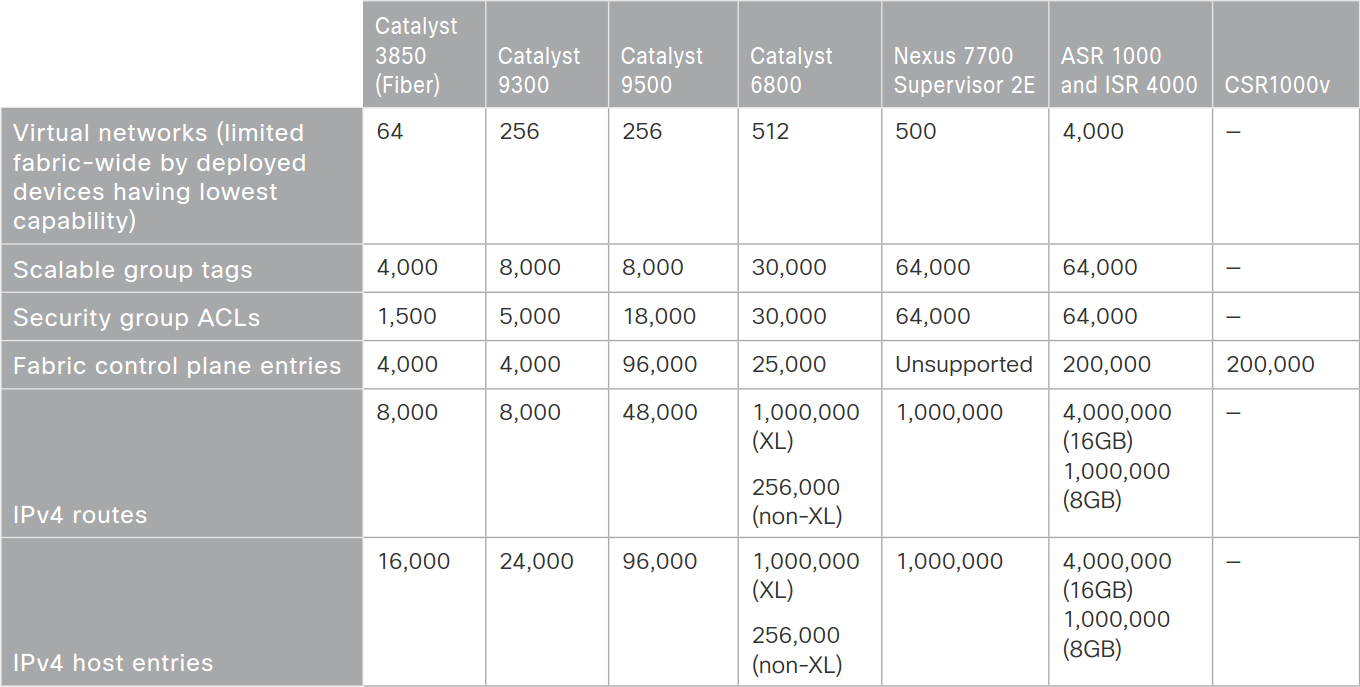
\includegraphics[width=1\linewidth]{img/MaximumScale-BorderNode.png}\\[1px]
	\caption{SDA Border Node Scale Constraints}
	\label{fig:SDA Border Node Scale Constraints}
\end{figure}

\pagebreak
\subsection{Verkabelungsplan}
\begin{longtable}{| l | l | l | l |}
		\hline
		\multicolumn{4}{| c| }{Verkabelung} \\
		\hline
		\multicolumn{2}{| c |}{Seite A} & \multicolumn{2}{ c |}{Seite B} \\
		\hline
		isr4431-1.access & GE0/0/0 & WAN & -\\
		\hline
		isr4431-1.access & GE0/0/1 & isr4431-2.access & GE0/0/1 \\
		\hline
		isr4431-1.access & GE0/0/2 & c9300-1.dist & GE1/0/1 \\
		\hline
		isr4431-2.access & GE0/0/0 & WAN & - \\
		\hline
		isr4431-2.access & GE0/0/1 & isr4431-1.access & GE0/0/1 \\
		\hline	
		isr4431-2.access & GE0/0/2 & c9300-2.dist & GE1/0/1 \\
		\hline			
		c9300-1.dist & GE1/0/2 & c9300-2.dist & GE1/0/2  \\
		\hline
		c9300-1.dist & GE1/0/3 & isr4431-1.core & GE0/0/0 \\
		\hline
		c9300-2.dist & GE1/0/3 & isr4431-2.core & GE0/0/0 \\
		\hline
		c9300-2.dist & GE1/0/4 & HSR Lab & - \\
		\hline
		isr4431-1.core & GE0/0/1 & isr4431-2.core & GE0/0/1 \\
		\hline
		isr4431-1.core & GE0/0/2 & c3850.g1.dist & GE1/0/1 \\
		\hline
		isr4431-1.core & GE0/0/3 & c3850.g2.access & GE1/0/1 \\
		\hline
		isr4431-1.core & GE0/1/0 & c9300.g3.access & GE1/0/1 \\
		\hline
		isr4431-2.core & GE0/0/2 & c3850.g1.dist & GE2/0/1 \\
		\hline
		isr4431-2.core & GE0/0/3 & c3850.g2.access & GE1/0/2 \\
		\hline
		isr4431-2.core & GE0/1/0 & c9300.g3.access & GE1/0/2 \\
		\hline
		c3850.g1.dist & GE1/0/2 & c3850.g1.access & GE1/0/1 \\
		\hline
		c3850.g1.dist & GE2/0/2 & c9300.g1.access & GE1/0/1 \\
		\hline
		c3850.g1.access & GE1/0/3 & c3650.g1.access & GE0/1 \\
		\hline
\end{longtable}


\subsection{Access Control Policies}

\paragraph{Virtual Network}
Virtuelle Netzwerke sind isolierte Routing- und Switching-Umgebungen. Standardmässig können Hosts die in seperaten virtuellen Netzwerken existieren nicht miteinander kommunizieren. Mit Hilfe von virtuellen Netzwerken kann das physische Netzwerk in mehrere logische Netzwerk geteilt werden. Ein typischer Anwendungsfall ist die Segmentierung von Gästen, Mitarbeitern und Kontraktor in getrennte Gruppen, so dass der Zugriff nur auf Teile des Netzwerkes erlaubt oder eingeschränkt werden kann. Die verschiedenen Arten von Netzwerken sind:

\begin{itemize}
	\item Gast-Netzwerk: Netzwerkverbindungen, die von einem Unternehmen zur Verfügung gestellt werden, um seinen Gästen den Zugang zum Internet und zum eigenen Unternehmen zu ermöglichen, ohne die Sicherheit des Host-Unternehmensnetzwerks zu beeinträchtigen. Gäste können auf das Internet zugreifen, aber nicht auf interne Anwendungen, die im Rechenzentrum gehostet werden.
	\item Mitarbeiter-Netzwerk: Netzwerkverbindungen, die den Zugriff auf das Internet und interne Anwendungen ermöglichen. Diese Gruppe kann weiter segmentiert werden, um z.B. den Zugriff innerhalb des Unternehmensnetzwerks zu ermöglichen oder einzuschränken, für bestimmte interne Anwendungen, Laborumgebungen und Server. Ein Finanzangestellter z.B. braucht keinen Zugang zum Entwicklungslabor. Ebenso benötigt ein Entwickler keinen Zugriff auf eine Verkaufsprognose. Diese können ohne Probleme in weitere virtuelle Netzwerke segmentiert werden.
	\item Kontraktor-Netzwerk: Netzwerkverbindung, die es den Benutzern ermöglicht, auf das Internet und auf unternehmensspezifische Anwendungen innerhalb des Unternehmensnetzwerks zuzugreifen. Ein virtuelles Netzwerk kann sich über mehrere Standorte und Netzwerkdomänen (Wireless, Campus und WAN) erstrecken.
\end{itemize}


\paragraph{Scalable Group}
Skalierbare Gruppen umfassen eine Gruppierung von Benutzern, Endgeräten oder Ressourcen, die dieselben Anforderungen an die Zugriffskontrolle stellen. Diese Gruppen (in Cisco ISE als Sicherheitsgruppen oder SGs bekannt) werden auf dem Cisco ISE definiert. Eine skalierbare Gruppe kann nur ein Element (ein Benutzer, ein Endgerät oder eine Ressource) enthalten.

\paragraph{Access Control Contract}
Ein Zugriffsvertrag ist eine Security Group Access Control List (SGACL). Sie definiert das Regelwerk, dass die Netzwerkinteraktion zwischen Quelle und Ziel in einer Zugriffskontrollrichtlinie regelt.

\paragraph{Group-based Access Control Policy}
Gruppenbasierte Zugriffskontrollrichtlinien sind Security Group Access Control Lists (SGACLs). DNA Center hat den Cisco ISE integriert, um den Prozess der Erstellung und Pflege von SGACLs zu vereinfachen. Während der initialen Integration von DNA Center und Cisco ISE werden skalierbare Gruppen und Richtlinien, die in Cisco ISE vorhanden sind, an das DNA Center weitergegeben und in das standardmäßige virtuelle Netzwerk eingefügt.

Das folgende Beispiel zeigt den Prozess der Authentifizierung und Zugriffskontrolle, den ein Benutzer durchläuft, wenn er sich in das Netzwerk einloggt:
\begin{enumerate}
	\item Ein Benutzer verbindet sich mit einem Port auf einem Switch und stellt seine Zugangsdaten zur Verfügung.
	\item Der Switch kontaktiert Cisco ISE.
	\item Cisco ISE authentifiziert den Benutzer und lädt die SGACLs auf den Port, mit dem der Benutzer verbunden ist.
	\item  Dem Benutzer wird der Zugang zu bestimmten Benutzern oder Geräten (Servern) auf der Grundlage des in die SGACL gewährt.
\end{enumerate}





\subsubsection{Workflow}
Workflow zur Konfiguration einer gruppenbasierten Zugriffskontrollrichtlinie.

\begin{table}[H]
	\rowcolors{2}{gray!25}{white}
	\centering
	\begin{tabularx}{\textwidth}{p{2 cm} | X | p{2 cm}}
		\rowcolor{gray!50}
		\textbf{Schritt} & \textbf{Aktion} & \textbf{Zweck} \\
		\hline	
		1 & Erstellen eines virtuellen Netzwerkes. Abhängig von der Konfiguration des Unternehmens und seinen Zugriffsanforderungen und -beschränkungen können die Gruppen in verschiedene virtuelle Netzwerke unterteilt werden, um eine weitere Segmentierung zu ermöglichen. & (Optional) \\
		2 & Erstellen einer skalierbaren Gruppe. Nach der Integration von Cisco ISE werden die in ISE vorhandenen skalierbaren Gruppen in das DNA Center übertragen. Wenn eine skalierbare Gruppe nicht besteht, kann diese direkt angelegt werden. & (Optional) \\
		3 & Erstellen eines Zugriffskontrollvertrag (access control contract). Ein Contract definiert eine Reihe von Regeln, die eine Aktion (erlauben oder verweigern), die Netzwerkgeräte basierend auf dem Datenverkehr durchführen, der bestimmten Protokollen oder Ports entspricht. & \\
		4 & Erstellen einer gruppenbasierten Zugriffskontrollrichtlinie (group-based access control policy). Die Zugriffskontrollrichtlinie definiert den Zugriffskontrollvertrag, der den Verkehr zwischen den skalierbaren Quell- und Zielgruppen regelt. & \\
		
	\end{tabularx}
	\caption{Workflow zur Erstellung der Access Control Policies}
	\label{tab:Workflow zur Erstellung der Access Control Policies}
\end{table}

\subsubsection{Erstellen eines virtuellen Netzwerkes}
\begin{enumerate}
	\item Wähle auf der DNA Center Homepage \textbf{Policy / Virtual Network}.
	\item Klicke auf den \textbf{Add Button} und fülle die erforderlichen Informationen aus.
	\item Klicke \textbf{Save}.
\end{enumerate}

\subsubsection{Erstellen einer Skalierbaren Gruppe}
\begin{enumerate}
	\item Wähle auf der DNA Center Homepage \textbf{Policy / Registry / Scalable Groups}. Alle skalierbaren Gruppen, die auf dem Cisco ISE erstellt wurden, erscheinen in der Registry.
	\item Klick \textbf{Add}. DNA Center öffnet eine direkte Verbindung zum Cisco ISE Server, wo die skalierbaren Gruppen hinzugefügt werden können.
	\item Erstelle in Cisco ISE skalierbare Gruppen (in Cisco ISE Sicherheitsgruppen genannt).
	\item Gehe zum DNA Center zurück. Nun sollte die erstellte skalierbare Gruppe angezeigt werden.
\end{enumerate}

\subsection{Erstellen eines Zugriffskontrollvertrages}
\begin{enumerate}
	\item Wähle auf der DNA Center Homepage \textbf{Policy / Contracts / Access Contracts}.
	\item Klick \textbf{Add Contract}.
	\item Im Dialogfenster des \textbf{Contract Editor} kann ein Namen und eine Beschreibung für den Vertrag erfasst werden.
	\item Wähle in der Dropdown-Liste \textbf{Implicit Action} entweder \textbf{Deny} oder \textbf{Permit}.
	\item Wähle aus der Dropdown-Lste in der Spalte \textbf{Port/Protocol} einen Port oder ein Protokoll aus. Hinweis: Wenn das DNA Center nicht über den Port oder das Protokoll verfügt welches benötigt wird, kann dies selbst erstellt werden. Klicke hierzu auf \textbf{Add Port/Protocol}, füge alle erforderlichen Informationen hinzu und klicke auf \textbf{Save}.
	\item (Optional) Um weitere Regeln in den Vertrag aufzunehmen, klicke auf \textbf{Add} und wiederhole Schritt 5 und 6.
	\item Klicke \textbf{Save}.
\end{enumerate}